\sloppy
\documentclass[14pt,a4paper,oneside]{extarticle}	% Размер основного шрифта и формата листа
\usepackage{xltxtra}						% Используется для вывода логотипа XeLaTeX
\usepackage{xunicode}						% Кодировка документа
\usepackage{polyglossia}					% Загружает пакет многоязыковой верстки
\newfontfamily\russianfont{Book Antiqua}
%\setmainfont{Liberation Serif}						% Основной шрифт текста
\setmainfont{Book Antiqua}
\setdefaultlanguage{russian}				% Основной язык текста
\setotherlanguage{english}					% Дополнительный язык текста
\linespread{1}							% Межстрочный интервал выбран полуторным
\usepackage[left=2.5cm,
right=1.5cm,vmargin=2.5cm]{geometry} % Отступы по краям листа
\bibliographystyle{ugost2008}

\usepackage{xcolor}
\usepackage{hyperref}
% Цвета для гиперссылок
\definecolor{linkcolor}{HTML}{359B08} % цвет ссылок
\definecolor{urlcolor}{HTML}{799B03} % цвет гиперссылок
\hypersetup{pdfstartview=FitH,  linkcolor=linkcolor,urlcolor=urlcolor, colorlinks=true}

%---------------------------%
%---- Пакеты расширений ----%
%---------------------------%
\usepackage{xcolor}
\usepackage{hyperref}
% Цвета для гиперссылок
\definecolor{linkcolor}{HTML}{359B08} % цвет ссылок
\definecolor{urlcolor}{HTML}{799B03} % цвет гиперссылок
\hypersetup{pdfstartview=FitH,  linkcolor=linkcolor,urlcolor=urlcolor, colorlinks=true}


\usepackage{verbatim,indentfirst}
\usepackage{cite,enumerate,float}
\usepackage{amsmath,amssymb,amsthm,amsfonts}

%---------------------------%
%--- Вставка иллюстраций ---%
%---------------------------%
\usepackage{graphicx}
\usepackage{subfigure}
\usepackage{fontspec}
%\graphicspath{{Images/}}

\begin{document}
%\pagestyle{empty} %  выключаенм нумерацию
%\setcounter{page}{3}% Нумерация начинается с третьей страницы
%\renewcommand{\contentsname}{\center{Содержание}}
%\tableofcontents

\newpage
\begin{center}
	%\addcontentsline{toc}{section}{Опыт 3. Третий закон Ньютона на примере силы Архимеда}
	\subsection*{Третий закон Ньютона на примере силы Архимеда}
\end{center}

\begin{figure}[H]
	\centering 		
	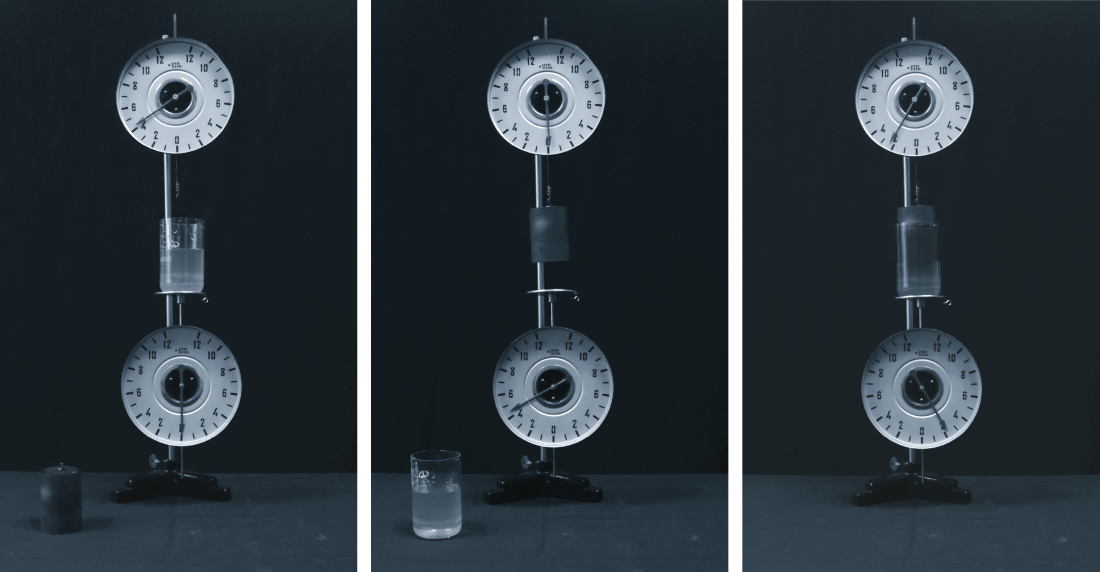
\includegraphics[width=1\linewidth]{newton-3.png} 
	\caption{Демонстрация третьего закона Ньютона}
	\label{newton-3}
\end{figure}

\subsection*{\underline{Оборудование:}}

\begin{enumerate}
	\item Физический штатив
	\item Динамометры демонстрационные с круглой шкалой до 1.2 кг для измерения сил
	\item Стакан с водой
	\item Цилиндр из эбонита с подвесом
\end{enumerate}

\newpage
\subsection*{\underline{Основные определения:}}

Пусть тело \textit{А} действует на другое тело \textit{В} с некоторой силой $\textbf{F}_1$. 
Тогда обязательно должна существовать ответная сила $\textbf{F}_2$, с которой 
тело \textit{В} будет действовать на тело \textit{А}.
При этом сила $\textbf{F}_2$ должна быть численно равна силе $\textbf{F}_1$, действовать вдоль той же прямой, но в противоположном силе $\textbf{F}_1$ направлении. 

Этот вывод позволяет дать третьему закону Ньютона очень 
простое количественное выражение: 
\textit{\begin{flushleft}
если какое-то тело действует на другое с силой $\textbf{F}_1$ то второе тело 
всегда действует на первое с ответной силой $\textbf{F}_2$, равной по модулю 
силе $\textbf{F}_1$ и противоположной ей по направлению: 
\end{flushleft}}
$$
\textbf{F}_{2} = - \textbf{F}_{1}
$$

В механике понятие веса является совершенно лишним. 
Но так как это слово простое, привычное, то им часто пользуются. 
Весом называют силу, с которой тело, находящееся только 
под влиянием силы тяжести, действует на подвес или на горизонтальную подставку, неподвижные в выбранной системе отсчета. 

Для неподвижных тела и опоры вес тела численно равен действующей на него силе тяжести, то есть $ \textbf{Р} = m\textbf{g} $, 
где \textit{m} — масса тела, \textbf{g} — ускорение свободного падения (или ускорение силы тяжести).
Поскольку масса тела — величина постоянная (в обычных условиях), а величина \textbf{g} изменяется на Земле с широтой и высотой над уровнем моря, то соответственно при этом изменяется и вес тела.
Одновременно значение \textbf{g}, а с ним и вес зависят от ускорения, обусловленного вращением 
Земли вокруг своей оси; по этой причине вес тела на экваторе меньше, чем на полюсе. 

В малой области вблизи земной поверхности значение \textbf{g} можно считать постоянным и 
вес тела — пропорциональным его массе, чем пользуются для измерения массы тел путем их 
взвешивания на рычажных весах; при этом значение \textbf{g} для взвешиваемого тела и гирь 
считается одним и тем же. 

Вес и масса являются разными физическими величинами, которые нельзя отождествлять;
они измеряются в разных единицах: вес — в единицах силы (Н, кгс, и др.), 
а масса — в единицах массы (кг, г, и др.).

Закон  Архимеда — закон статики жидкостей и газов, согласно которому на всякое тело, погруженное в жидкость (или газ), действует со стороны этой жидкости (газа) поддерживающая сила, равная весу вытесненной телом жидкости (газа), направленная вверх и приложенная к центру тяжести вытесненного объема.
Поддерживающую силу называют также архимедовой, или гидростатической подъемной силой. 
Давление, действующее на погруженное в жидкость тело, увеличивается с глубиной погружения, поэтому сила давления жидкости на нижние элементы поверхности тела больше, чем на верхние. 
В результате сложения всех сил, действующих на каждый элемент поверхности, получается равнодействующая $ \textbf{F} $, направленная вверх. Это и есть поддерживающая сила.

Если тело плотно лежит на дне, то давление жидкости только сильнее прижимает его ко дну. 
Если вес тела меньше поддерживающей силы, тело всплывает на поверхность жидкости до тех пор, пока вес вытесненной погруженной частью тела жидкости не станет равным поддерживающей силе. 
Если вес тела больше поддерживающей силы, тело тонет; если же вес тела равен поддерживающей силе, тело плавает внутри жидкости.

\newpage
\subsection*{\underline{Краткое описание демонстрации:}}

Для демонстрации третьего закона Ньютона требуется пара динамометров, стакан с жидкостью, и тело цилиндрической формы.

Если подвесить тело цилиндрической формы к крючку верхнего динамометра (рис.\ref{newton-3}), то стрелка динамометра зарегистрирует вес цилиндра.
Подобным образом по показаниям нижнего динамометра можно судить о величине давления оказываемого стаканом на опору.

В ходе опыта осуществлялась калибровка динамометров таким образом, чтобы стрелка нагруженного динамометра находилась в положении «0».
При взвешивании цилиндра, частично погруженного в жидкость, абсолютные показания обоих динамометров совпадают, однако стрелки отклонятся в противоположные стороны.
Динамометр, к которому подвешен груз, покажет уменьшение веса тела (отклонение стрелки влево), а нижний динамометр, на котором располагается стакан, будет демонстрировать увеличение веса (отклонение стрелки вправо).

\textit{Устройство динамометров}. Динамометр изготовлен в виде круглого металлического кожуха, на задней стенке которого имеется механизм из двух спиральных пружин и оси динамометра с зубчатой передачей; механизм закрыт металлической коробкой.
Ось динамометра соединена зубчаткой со стрелкой. 
Концы оси выходят из коробки, закрывающей механизм, вверх и вниз.
При действии силы на ось (сверху или снизу), стрелка динамометра отклоняется влево или вправо.

Посредством металлического стержня каждый динамометр укрепляется на стойке физического штатива.

Оси можно придавать любое направление, поворачивая динамометр в муфте штатива, на котором он укреплен.
На осях около коробки кожуха находятся корректоры, позволяющие регулировать механизм динамометра.

Шкала имеет влево и вправо от нуля до 12 делений ценою 100 г каждое.
Таким образом вся шкала рассчитана на нагрузку 1.2 кг.
Цифры обозначены на шкале через каждые 200 г условно в целых числах: 0, 2, 4, 6, 8, 10, 12; каждое число принимается за количество сотен граммов.
Циферблат может с легким трением вращаться относительно кожуха и стрелки, что дает возможность быстро и удобно устанавливать стрелку прибора на нуль шкалы в различных положениях.

\textit{Регулировка прибора}. Регулировка показаний динамометра производится специальными корректорами, сквозь которые проходит ось прибора.
Поворотом верхней и нижней гаек изменяют число рабочих витков пружины, после чего производят постепенную нагрузку динамометра точными гирями от 100 до 1200 г, чтобы проверить его показания по всей шкале.

\newpage
\subsection*{\underline{Теория:}}

Архимедова сила действует на всякое тело погруженное в жидкость, или газ.
Для того чтобы выяснить причину возникновения данной силы, рассмотрим цилиндр площадью поперечного сечения $ S $ и высотой $ h $, погруженный в жидкость плотности $\rho$ (рис.\ref{newton-4}). 
Основание цилиндра перпендикулярно вектору \textbf{g}. 
Верхняя граница цилиндра находится на высоте $ h_{1} $, нижняя — на глубине $ h_{2} = h_{1} + h $.

На боковую стенку цилиндра действуют силы давления, которые приводят к сжатию цилиндра.
Эти силы в условиях данного опыта можно не учитывать.

\begin{figure}[H] 
	\centering 	
	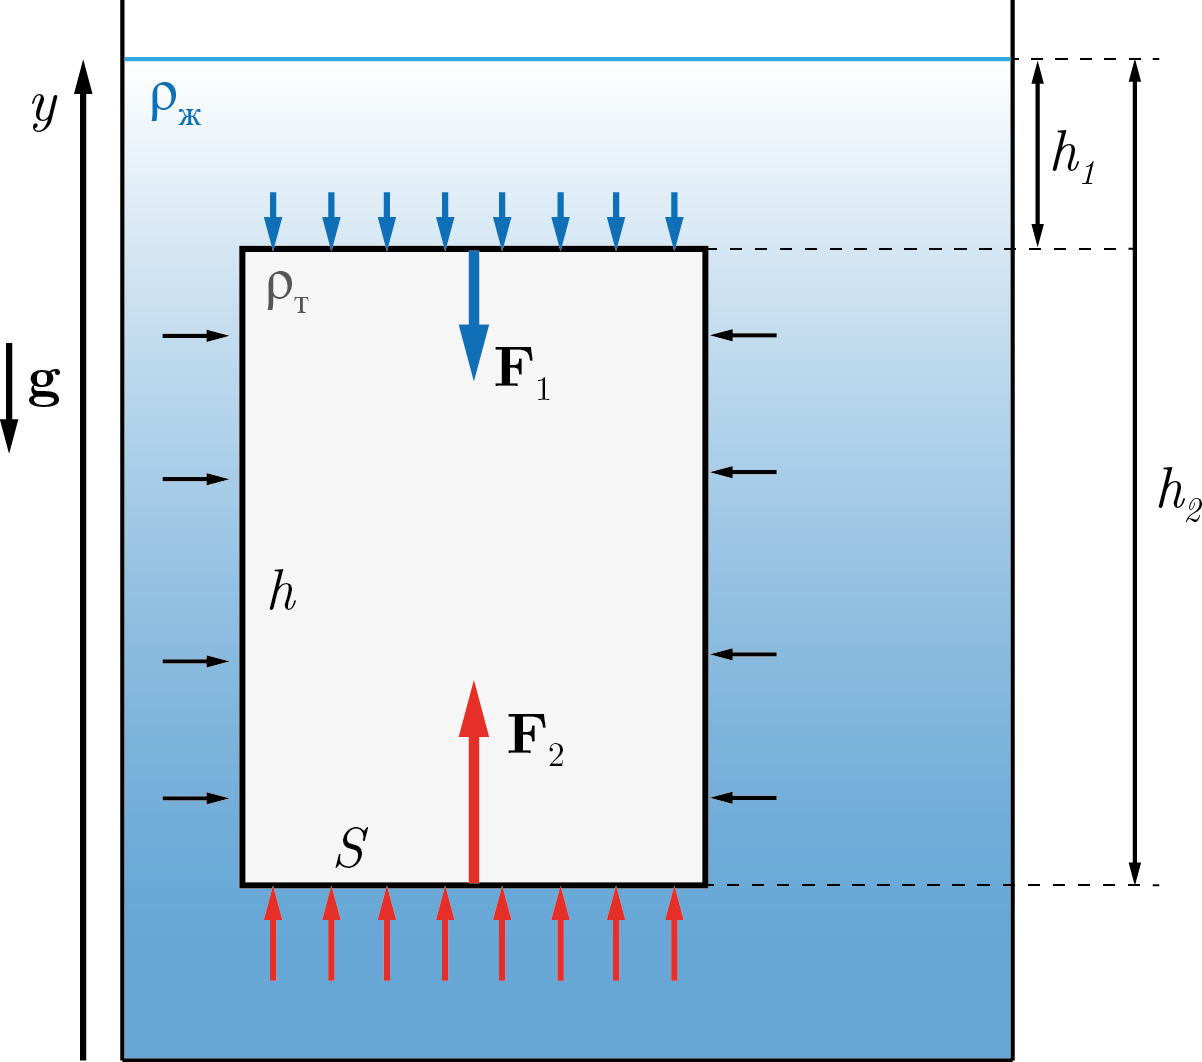
\includegraphics[width=0.5\linewidth]{newton-4.png}
	\caption{Схематическое изображение сил, действующее на погруженное в жидкость тело}
	\label{newton-4}
\end{figure}

На уровне верхнего основания цилиндра давление жидкости равно $$ p_{1} = \rho gh_{1}. $$

поэтому на него действует сила давления $$ F_{1} = p_{1}S = \rho gh_{1}S, $$
направленная вертикально вниз.

На уровне нижнего основания давление жидкости составляет $$p_{2} = \rho gh_{2}.$$

Сила давления в этом случае $$ F_{2} = p_{2}S = \rho gh_{2}S, $$ 
направлена вертикально вверх по закону Паскаля.

Так как $ h_{2} < h_{1} $, то $ F_{2} < F_{1} $, и поэтому возникает равнодействующая сил давления, направленная вверх. 
Это и есть архимедова сила $ F_{A} $. 

В проекции на вертикальную ось $ y $ имеем:
\begin{equation}\label{newton-eq7}
F_{A} = F_{2} - F_{1} = \rho gh_{2} - \rho gh_{1} = \rho g(h_{2} - h_{1}) = \rho gh
\end{equation} 
Так как произведение $ Sh $ равно объему тела, погруженного в жидкость, получаем: 
\begin{equation}\label{newton-eq8}
F_{A} = \rho gV
\end{equation} 

Это выражение позволяет вычислять силу Архимеда.
Появление выталкивающей силы обусловлено тем, что давление жидкости на нижнее основание цилиндра больше, чем на верхнее.

Выражение (\ref{newton-eq8}) можно интерпретировать следующим образом. 
Произведение $ \rho V $ обозначает массу жидкости  $ m = \rho V $. 
Тогда $$\rho g V = mg = P,$$
где $ P $ — вес жидкости взятой в объеме $ V $. 
Таким образом, имеем:
\begin{equation}\label{newton-eq9}
F_{A} = P,
\end{equation} 

причем 

\begin{equation}\label{newton-eq10}
\textbf{F}_{A} = -\textbf{P}.
\end{equation} 

Можно заключить, что архимедова сила, действующая на погруженный в жидкость цилиндр, численно равна весу жидкости, вытесненной этим цилиндром.
Векторы силы Архимеда и веса жидкости имеют противоположные направления, следовательно подчиняются третьему закону механики Ньютона.

\end{document}
